% !TeX spellcheck = en_US
\documentclass[11pt,fancy,authorye]{elegantbook}
\usepackage{xcolor}
\usepackage[utf8]{inputenc}
\usepackage[french]{babel}
\usepackage{algorithm}
\usepackage{algpseudocode}
% Custom definitions for French keywords in algorithmicx
\algrenewcommand\algorithmicif{\textbf{Si}}
\algrenewcommand\algorithmicelse{\textbf{Sinon}}
\algrenewcommand\algorithmicfor{\textbf{Pour}}
\algrenewcommand\algorithmicdo{\textbf{Faire}}
\algrenewcommand\algorithmicwhile{\textbf{Tant~que}}
%\algrenewcommand\algorithmicendwhile{\textbf{Fin Tant que}}
%\algrenewcommand\algorithmicelseif{\textbf{Sinon Si}}

\algrenewcommand\algorithmicthen{\textbf{Alors}}
\algrenewcommand\algorithmicend{\textbf{Fin}}
\algrenewcommand\algorithmicreturn{\textbf{Retour}}


\usepackage[T1]{fontenc}
%\usepackage{titletoc}
\usepackage{minitoc}
\usepackage{mdframed}
\usepackage{verbatim}
\usepackage{listings}
\lstset{% Formatting C codes
	language=C,
	basicstyle=\ttfamily,
	numbers=left,
	xleftmargin=1.5cm, % Adjust this value as needed
	xrightmargin=.5cm, % Adjust this value as needed
}


\definecolor{remarkcolor}{RGB}{255,128,0} % Define the color for "Remark"
% Define a command for chapter-wise mini tables of contents
%\newcommand{\chaptertoc}{%
%	\startcontents[chapters]
%	\printcontents[chapters]{}{1}{\section*{\contentsname}}
%	\vspace{1cm} % Adjust the spacing as needed
%}

\newtheorem{remarque}{Remarque}

\title{Kajy University: Informatique}
\subtitle{Algorithmes et structures de données}

\author{Dimby Rabearivony}
\date{\today}
\version{1.0}


\extrainfo{"Ny fahalalana no valamparihiko."}

\logo{Kajy U.png}
\cover{hay.jpg}
%\usepackage{minitoc}

\begin{document}
	
	\maketitle
	
	\frontmatter
	\tableofcontents
	
	\mainmatter
	\chapter*{Introduction}

\noindent ``En fait, je dirai que la différence entre un mauvais programmeur et un bon réside dans le fait qu'il considère son code ou ses structures de données comme plus importants. Les mauvais programmeurs se soucient du code. Les bons programmeurs se soucient des structures de données et de leurs relations.''

\hfill - Linus Torvalds
	\chapter{Structures de donn\'ees fondamentales}
%\minitoc
\section{Variables}
Les variables constituent l'un des concepts les plus fondamentaux en programmation. En langage C, une variable est un espace de stockage nommé qui peut contenir une valeur modifiable. Les variables sont utilisées pour stocker des données telles que des nombres, des caractères et des adresses mémoire.

\subsection{Déclaration de variables}

En language C, on d\'eclare une variable en pr\'ec\'edant son nom le type de donn\'ee qu'elle contient. 

\begin{lstlisting}
	int age; // Declaration d'une variable de type entier appelee "age"
	float prix; // Declaration d'une variable de type flottant appelee "prix"
	char lettre; // Declaration d'une variable de type caractere appelee "lettre"
\end{lstlisting}

\subsection{Initialisation des variables}

Les variables peuvent être initialisées lors de leur déclaration en leur attribuant une valeur initiale. Par exemple :

\begin{lstlisting}
	int nombre = 10; // Declaration et initialisation d'une variable de type entier avec la valeur 10
	float pi = 3.14; // Declaration et initialisation d'une variable de type flottant avec la valeur 3.14
	char grade = 'A'; // Declaration et initialisation d'une variable de type caractere avec la valeur 'A'
\end{lstlisting}

\subsection{Utilisation des variables}

Une fois déclarées et éventuellement initialisées, les variables peuvent être utilisées dans le programme pour stocker et manipuler des données. Par exemple :

\begin{lstlisting}
	#include <stdio.h>;
	int x = 5;
	int y = 10;
	int somme = x + y; // Addition des valeurs des variables x et y
	printf("La somme de %d et %d est %d\n", x, y, somme); // Affichage du resultat
\end{lstlisting}

\subsection{Portée des variables}

La portée d'une variable en C détermine où elle peut être utilisée dans le programme. Les variables peuvent être locales à une fonction, auquel cas elles ne sont accessibles que dans cette fonction, ou elles peuvent être globales, auquel cas elles sont accessibles dans tout le programme.

\begin{lstlisting}
	#include <stdio.h>;
	
	int globalVar = 100; // Variable globale
	
	void exampleFunction() {
		int localVar = 50; // Variable locale a la fonction exampleFunction
		printf("La variable globale est %d\n", globalVar); // Acces a la variable globale
		printf("La variable locale est %d\n", localVar); // Acces a la variable locale
	}
	
	int main() {
		printf("La variable globale est %d\n", globalVar); // Acces a la variable globale
		// printf("La variable locale est %d\n", localVar); // Cela generera une erreur car localVar est locale a exampleFunction
		exampleFunction();
		return 0;
	}
\end{lstlisting}

Les variables sont un element essentiel en langage C et constituent la base de la manipulation des donnees dans les programmes. Il est crucial de comprendre leur declaration, leur initialisation, leur utilisation et leur portee pour ecrire des programmes efficaces et fonctionnels.


\section{Pointeurs}

Les pointeurs sont un concept essentiel en langage C. Un \emph{pointeur} est une variable qui contient l'adresse mémoire d'une autre variable. En d'autres termes, un pointeur pointe vers l'emplacement en mémoire où une valeur est stockée.

\subsection{Déclaration de pointeurs}

En langage C, un pointeur est déclaré en précédant le nom de la variable avec l'opérateur *, qui indique que la variable est un pointeur. Voici un exemple de déclaration de pointeur :

\begin{lstlisting}
	int *ptr; // Declaration d'un pointeur vers un entier
	float *ptr_float; // Declaration d'un pointeur vers un flottant
	char *ptr_char; // Declaration d'un pointeur vers un caractere
\end{lstlisting}

\subsection{Initialisation de pointeurs}

Les pointeurs peuvent être initialisés avec l'adresse mémoire d'une variable existante à l'aide de l'opérateur d'adresse \&. Voici un exemple d'initialisation de pointeur :

\begin{lstlisting}
	int var = 10; // Declaration et initialisation d'une variable
	int *ptr; // Declaration d'un pointeur
	ptr = &var; // Initialisation du pointeur avec l'adresse de la variable var
\end{lstlisting}

\subsection{Utilisation de pointeurs}

Une fois qu'un pointeur est initialisé, il peut être utilisé pour accéder à la valeur à laquelle il pointe ou pour modifier cette valeur. Voici quelques exemples :

\begin{lstlisting}
	#include <stdio.h>;
	int var = 10; // Declaration et initialisation d'une variable
	int *ptr; // Declaration d'un pointeur
	ptr = &var; // Initialisation du pointeur avec l'adresse de la variable var
	printf("La valeur de var est %d\n", var); // Affichage de la valeur de var
	printf("L'adresse de var est %p\n", &var); // Affichage de l'adresse de var
	printf("La valeur pointee par le pointeur est %d\n", *ptr); // Affichage de la valeur pointee par le pointeur
	*ptr = 20; // Modification de la valeur pointee par le pointeur
	printf("La nouvelle valeur de var est %d\n", var); // Affichage de la nouvelle valeur de var
\end{lstlisting}

Les pointeurs sont un concept puissant en langage C, mais ils nécessitent une manipulation prudente pour éviter les erreurs de segmentation et les fuites de mémoire.

\subsection{Double pointeurs}

Les double pointeurs (ou pointeurs vers des pointeurs) contiennent l'adresse mémoire d'un autre pointeur. Ils sont utiles pour passer des pointeurs par référence à des fonctions, pour des structures de données complexes comme des tableaux de tableaux, ou pour manipuler des listes chaînées.

Voici un exemple de déclaration et d'utilisation d'un double pointeur :

\begin{lstlisting}
	int a = 5;
	int *ptr = &a; // Pointeur vers int
	int **double_ptr = &ptr; // Double pointeur vers pointeur int
	
	printf("La valeur de a est %d\\n", a); // Affichage de la valeur de a
	printf("La valeur pointe par ptr est %d\\n", *ptr); // Affichage de la valeur pointee par ptr
	printf("La valeur pointee par double_ptr est %d\\n", **double_ptr); // Affichage de la valeur pointee par double_ptr
\end{lstlisting}

Les double pointeurs sont également utilisés pour retourner des pointeurs depuis des fonctions ou pour allouer dynamiquement de la mémoire pour des structures comme des tableaux 2D.

\subsection{Utilisation avancée des pointeurs}

Les pointeurs permettent des opérations avancées comme l'arithmétique des pointeurs, où vous pouvez ajouter ou soustraire des valeurs pour déplacer le pointeur en mémoire. Voici un exemple :

\begin{lstlisting}
	int tableau[5] = {1, 2, 3, 4, 5};
	int *ptr = tableau;
	
	printf("Premier element: %d\\n", *ptr); // Affichage du premier element
	ptr++; // Deplacement du pointeur vers le prochain element
	printf("Deuxieme element: %d\\n", *ptr); // Affichage du deuxieme element
\end{lstlisting}

Soyez prudent avec l'arithmétique des pointeurs, car elle peut conduire à des erreurs de segmentation si vous sortez des limites de la mémoire allouée.

\subsection{Pointeurs et mémoire dynamique}

Les pointeurs sont essentiels pour la gestion de la mémoire dynamique en langage C. Avec des fonctions comme `malloc` et `free`, vous pouvez allouer et libérer de la mémoire au moment de l'exécution. Voici un exemple :

\begin{lstlisting}
	int *array = (int *)malloc(10 * sizeof(int)); // Allouer de la memoire pour 10 entiers
	if (array == NULL) {
		printf("Echec de l'allocation de memoire!\\n");
		return 1;
	}
	
	for (int i = 0; i < 10; i++) {
		array[i] = i * 2; // Initialisation de la memoire allouee
	}
	
	free(array); // Liberer la memoire
\end{lstlisting}

La gestion de la mémoire est cruciale lors de l'utilisation des pointeurs. Assurez-vous de toujours libérer la mémoire allouée pour éviter les fuites de mémoire.


\section{Types de données}

Les types de données en langage C déterminent la nature des valeurs qu'une variable peut contenir. Le langage C prend en charge plusieurs types de données de base, ainsi que des types de données dérivés tels que les tableaux et les structures.

\subsection{Types de données de base}

Les types de données de base définissent les valeurs simples que peuvent contenir les variables en langage C. Voici quelques-uns des types de données de base les plus couramment utilisés, avec leurs tailles habituelles:

\begin{enumerate}[label=\alph*)]
	\item \textbf{int} : Pour les entiers signés (généralement 4 octets).
	\item \textbf{float} : Pour les nombres à virgule flottante (généralement 4 octets).
	\item \textbf{double} : Pour les nombres à virgule flottante double précision (généralement 8 octets).
	\item \textbf{char} : Pour les caractères ASCII (généralement 1 octet).
\end{enumerate}

Voici des exemples de déclaration de variables pour ces types de données:

\begin{lstlisting}
	int age = 30; // Declaration d'une variable de type entier
	float poids = 75.5; // Declaration d'une variable de type flottant
	double prix = 99.99; // Declaration d'une variable de type double
	char grade = 'A'; // Declaration d'une variable de type caractere
\end{lstlisting}

\subsection{Types de données dérivés}

Outre les types de données de base, le langage C offre la possibilité de créer des types de données dérivés, comme les tableaux, les structures, les unions et les énumérations.

\begin{enumerate}[label=\alph*)]
	\item \textbf{Tableaux} :
	
	Un tableau est une collection ordonnée d'éléments du même type. Les éléments d'un tableau sont accessibles via un index numérique. Voici un exemple de déclaration d'un tableau et d'opérations de base:
	
	\begin{lstlisting}
		int tableau[5]; // Declaration d'un tableau de taille 5
		tableau[0] = 10; // Attribuer la valeur 10 au premier element
		tableau[1] = 20; // Attribuer la valeur 20 au deuxieme element
	\end{lstlisting}
	
	\item \textbf{Structures} :
	
	Les structures permettent de regrouper des variables de types différents. Elles permettent de définir des types de données personnalisés. Voici un exemple d'utilisation des structures:
	
	\begin{lstlisting}
		#include <stdio.h>;
		#include <string.h>;
		
		struct Personne {
			char nom[50];
			int age;
			float taille;
		};
		
		struct Personne p1; // Declaration d'une structure de type Personne
		strcpy(p1.nom, "John Doe"); // Attribution d'une valeur au champ nom
		p1.age = 30; // Attribution d'une valeur au champ age
		p1.taille = 1.75; // Attribution d'une valeur au champ taille
	\end{lstlisting}
	
	\item \textbf{Unions} :
	
	Les unions permettent de partager la même zone mémoire entre différents types de données. Voici un exemple de déclaration d'une union:
	
	\begin{lstlisting}
		union Data {
			int entier;
			float flottant;
			char caractere;
		};
		
		union Data d;
		d.entier = 10; // Utilisation de l'union avec un entier
		d.flottant = 5.5; // Utilisation avec un flottant (ecrase l'entier)
	\end{lstlisting}
	
	\item \textbf{Énumérations} :
	
	Les énumérations permettent de définir un ensemble de valeurs nommées. Elles sont utiles pour créer des listes de constantes. Voici un exemple d'utilisation des énumérations:
	
	\begin{lstlisting}
		enum Jour {LUNDI, MARDI, MERCREDI, JEUDI, VENDREDI, SAMEDI, DIMANCHE};
		
		enum Jour aujourdhui = MERCREDI; // Declaration d'une enumeration et initialisation
	\end{lstlisting}
\end{enumerate}

\subsection{Typedef}

Le mot-clé \emph{typedef} permet de créer des alias pour des types de données existants. Cela peut simplifier des déclarations complexes, rendre le code plus lisible, et améliorer l'abstraction des types. `typedef` est couramment utilisé pour simplifier des déclarations de pointeurs, de structures, d'unions, et de fonctions.

\subsubsection*{Alias pour des types de base}

Voici un exemple d'utilisation de `typedef` pour créer un alias pour un type de base :

\begin{lstlisting}
	typedef int Entier; // Creation d'un alias pour int
	Entier age = 30; // Utilisation du typedef pour creer un alias
\end{lstlisting}

Cet exemple montre comment `typedef` peut simplifier des déclarations. Utiliser des alias descriptifs peut rendre le code plus lisible et compréhensible, en particulier lorsque les types de base ont des applications spécifiques.

\subsubsection*{Utilisation avec des pointeurs}

Les pointeurs en C peuvent être complexes à déclarer, surtout pour les pointeurs de fonctions ou les structures dérivées. `typedef` simplifie les déclarations de pointeurs en créant des alias :

\begin{lstlisting}
	typedef int* PointeurEntier; // Alias pour un pointeur vers int
	PointeurEntier ptr = NULL; // Declaration d'un pointeur vers int
\end{lstlisting}

Vous pouvez également utiliser `typedef` pour simplifier des déclarations de pointeurs de fonctions, rendant le code plus lisible :

\begin{lstlisting}
	typedef int (*Fonction)(int, int); // Alias pour un pointeur vers une fonction
\end{lstlisting}

\subsubsection*{Utilisation avec des structures}

`typedef` est largement utilisé pour simplifier les déclarations de structures complexes. Cela facilite l'utilisation de structures pour regrouper des variables de types différents :

\begin{lstlisting}
	typedef struct {
		char nom[50];
		int age;
		float taille;
	} Personne;
	
	Personne p1; // Utilisation du typedef pour nommer une structure
\end{lstlisting}

Avec `typedef`, les déclarations de structures deviennent plus concises et lisibles, ce qui peut simplifier le code et faciliter les modifications futures.

\subsubsection*{Utilisation avec des unions}

Les unions permettent de partager la même zone mémoire entre différents types de données. `typedef` peut être utilisé pour nommer des unions, ce qui simplifie l'utilisation des structures complexes :

\begin{lstlisting}
	typedef union {
		int entier;
		float flottant;
		char caractere;
	} Donnees;
	
	Donnees d; // Utilisation du typedef pour nommer une union
\end{lstlisting}

\subsubsection*{Utilisation avec des énumérations}

Les énumérations permettent de définir des ensembles de valeurs nommées. `typedef` facilite la déclaration et l'utilisation des énumérations :

\begin{lstlisting}
	typedef enum {LUNDI, MARDI, MERCREDI, JEUDI, VENDREDI, SAMEDI, DIMANCHE} Jour;
	
	Jour aujourdhui = MERCREDI; // Utilisation de l'enumeration avec typedef
\end{lstlisting}

\subsubsection*{Avantages de `typedef`}

`typedef` offre plusieurs avantages pour le code C, notamment :

- \textbf{Simplification des déclarations complexes} : `typedef` permet de rendre le code plus concis en créant des alias pour des déclarations compliquées.
- \textbf{Lisibilité accrue} : Les alias créés avec `typedef` rendent le code plus facile à lire et à comprendre.
- \textbf{Abstraction des types} : `typedef` permet de créer des abstractions pour des types de données, ce qui facilite les modifications futures.
- \textbf{Réutilisation du code} : Les alias créés avec `typedef` peuvent être réutilisés dans différents contextes, ce qui améliore la maintenabilité du code.

Dans l'ensemble, `typedef` est un outil puissant en langage C qui permet de simplifier les déclarations complexes, de rendre le code plus lisible, et de faciliter la création de types de données personnalisés. Que ce soit pour des pointeurs, des structures, des unions, ou des fonctions, `typedef` est un outil précieux pour les développeurs C.


%\section{Exercices}
%
%\textbf{Types de données:}
%
%\begin{enumerate}
%	\item Écrivez un programme C pour déclarer une variable de chaque type de données de base et initialisez-les avec des valeurs.
%	\item Déclarez un tableau d'entiers de taille 10 et initialisez-le avec des valeurs de votre choix. Affichez ensuite ces valeurs à l'écran.
%	\item Créez une structure \texttt{Personne} avec des champs pour le nom, l'âge et la taille. Déclarez une variable de type \texttt{Personne} et initialisez-la avec des valeurs fictives. Affichez ensuite ces valeurs à l'écran.
%%	\item Écrivez une fonction en C pour inverser une chaîne de caractères donnée.
%%	\item Écrivez une fonction en C pour trier un tableau d'entiers en utilisant l'algorithme de tri à bulles.
%%\end{enumerate}
%
%\textbf{Types de données de base:}
%
%%\begin{enumerate}
%	
%	\item Écrivez une fonction en C pour calculer la somme des chiffres d'un nombre entier.
%	\item Déclarez une variable de type \texttt{char} et utilisez-la pour stocker une lettre majuscule. Ensuite, utilisez une opération pour convertir cette lettre en minuscule.
%	\item Écrivez un programme C pour vérifier si un nombre donné est premier ou non.
%	\item Écrivez une fonction récursive en C pour calculer le factoriel d'un nombre entier.
%	\item Écrivez un programme C pour convertir un nombre entier en binaire.
%%\end{enumerate}
%
%\textbf{Types de données dérivés:}
%
%%\begin{enumerate}
%	\item Écrivez une fonction en C pour concaténer deux chaînes de caractères données.
%	\item Déclarez un tableau de structures \texttt{Etudiant} avec des champs pour le nom, l'âge et la moyenne. Initialisez-le avec des valeurs fictives et affichez ensuite ces valeurs à l'écran.
%	\item Écrivez une fonction en C pour ajouter un élément à une liste chaînée.
%	\item Implémentez une file (queue) en utilisant des listes chaînées en C.
%	\item Écrivez une fonction en C pour supprimer un élément d'un arbre binaire de recherche.
%%\end{enumerate}
%
%\textbf{Typedef}
%
%%\begin{enumerate}
%	 \item \textbf{Création d'un alias pour un type de base}
%	
%	Utilisez `typedef` pour créer un alias pour un type de données de base. Ensuite, déclarez une variable de ce type et affichez sa valeur.
%	
%	\begin{lstlisting}
%		typedef ...
%		... var = 25;
%		
%		printf("La valeur de var est %d\\n", var);
%	\end{lstlisting}
%	
%	\item \textbf{Utilisation de typedef avec des pointeurs}
%	
%	Utilisez `typedef` pour créer un alias pour un pointeur vers un entier. Initialisez le pointeur avec l'adresse d'une variable entière et affichez la valeur à laquelle le pointeur fait référence.
%	
%	\begin{lstlisting}
%		typedef ...
%		int a = 10;
%		... ptr = &a;
%		
%		printf("La valeur pointee par le pointeur est %d\\n", *ptr);
%	\end{lstlisting}
%	
%	\item \textbf{Utilisation de typedef avec des structures}
%	
%	Utilisez `typedef` pour créer un alias pour une structure représentant une personne avec des champs comme le nom, l'âge, et la taille. Ensuite, déclarez une variable de ce type et attribuez des valeurs aux champs.
%	
%	\begin{lstlisting}
%		typedef struct {
%			char nom[50];
%			int age;
%			float taille;
%		} ...;
%		
%		... p1;
%		
%		strcpy(p1.nom, "Alice");
%		p1.age = 25;
%		p1.taille = 1.65;
%	\end{lstlisting}
%	
%	\item \textbf{Utilisation de typedef avec des énumérations}
%	
%	Utilisez `typedef` pour créer un alias pour une énumération représentant les jours de la semaine. Déclarez une variable de ce type et attribuez-lui un jour spécifique.
%	
%	\begin{lstlisting}
%		typedef enum {
%			LUNDI,
%			MARDI,
%			MERCREDI,
%			...
%		} ...;
%		
%		... aujourd'hui = MERCREDI;
%	\end{lstlisting}
%	
%	\item \textbf{Utilisation de typedef avec des unions}
%	
%	Utilisez `typedef` pour créer un alias pour une union contenant un entier, un flottant, et un caractère. Déclarez une variable de ce type et attribuez des valeurs aux différents éléments de l'union.
%	
%	\begin{lstlisting}
%		typedef union {
%			int entier;
%			float flottant;
%			char caractere;
%		} ...;
%		
%		... d;
%		d.entier = 10;
%		d.flottant = 5.5;
%	\end{lstlisting}
%\end{enumerate}

\section{Exercices}

\subsection{Variables et types de données}
\begin{enumerate}
	\item Quelle est la différence entre les types de données suivants :
	\begin{enumerate}
		\item \textbf{int}
		\item \textbf{float}
		\item \textbf{char}
	\end{enumerate}
	
	\item Écrivez un programme C qui déclare des variables pour chaque type de données mentionné et affiche leurs valeurs.
	% \textbf{Réponse:}
	% \begin{lstlisting}
		% #include <stdio.h>
		
		% int main() {
			%     int entier = 42; 
			%     float flottant = 3.14; 
			%     char caractere = 'A'; 
			
			%     printf("Entier: %d\n", entier);
			%     printf("Flottant: %.2f\n", flottant);
			%     printf("Caractère: %c\n", caractere);
			
			%     return 0;
			% }
		% \end{lstlisting}
	
	\item Écrivez un programme C qui utilise des variables de différents types de données pour calculer la somme d'un entier et d'un flottant, puis affichez le résultat.
	% \textbf{Réponse:}
	% \begin{lstlisting}
		% #include <stdio.h>
		
		% int main() {
			%     int entier = 10;
			%     float flottant = 2.5;
			
			%     float somme = entier + flottant; 
			
			%     printf("La somme est: %.2f\n", somme);
			
			%     return 0;
			% }
		% \end{lstlisting}
	
	\item Quelles sont les limites de valeurs pour les types de données suivants :
	\begin{enumerate}
		\item \textbf{int}
		\item \textbf{float}
		\item \textbf{double}
	\end{enumerate}
	% \textbf{Réponse:}
	% a. `int`: généralement de `-2,147,483,648` à `2,147,483,647`.
	% b. `float`: de `1.2E-38` à `3.4E+38`.
	% c. `double`: de `2.3E-308` à `1.7E+308`.
\end{enumerate}

\subsection{Pointeurs}
\begin{enumerate}
	\item Quelle est la différence entre une variable et un pointeur ?
	\item Écrivez un programme C qui utilise des pointeurs pour modifier la valeur d'une variable.
	% \textbf{Réponse:}
	% \begin{lstlisting}
		% #include <stdio.h>
		
		% int main() {
			%     int x = 10;
			%     int *p = &x; 
			
			%     printf("Valeur de x avant modification: %d\n", x);
			
			%     *p = 20;
			
			%     printf("Valeur de x après modification: %d\n", x);
			
			%     return 0;
			% }
		% \end{lstlisting}
	
	\item Écrivez un programme C qui utilise des pointeurs pour échanger les valeurs de deux variables.
	% \textbf{Réponse:}
	% \begin{lstlisting}
		% #include <stdio.h>
		
		% void echanger(int *a, int *b) {
			%     int temp = *a;
			%     *a = *b;
			%     *b = temp;
			% }
		
		% int main() {
			%     int x = 10;
			%     int y = 20;
			
			%     printf("Avant l'échange: x = %d, y = %d\n", x, y);
			
			%     echanger(&x, &y);
			
			%     printf("Après l'échange: x = %d, y = %d\n", x, y);
			
			%     return 0;
			% }
		% \end{lstlisting}
	
	\item Expliquez ce qu'est un pointeur nul (null pointer) et ce qui se passe si vous tentez d'utiliser un pointeur nul.
	% \textbf{Réponse:} Un pointeur nul (`NULL`) ne pointe pas vers une adresse mémoire valide. Tenter d'utiliser ou de déréférencer un pointeur nul peut provoquer des erreurs de segmentation ou des plantages du programme.
\end{enumerate}

\subsection{Tableaux}
\begin{enumerate}
	\item Déclarez un tableau de 5 entiers et initialisez-le avec des valeurs. Écrivez un programme C pour afficher les valeurs du tableau.
	\item Modifiez le programme pour inverser les éléments du tableau et afficher le tableau inversé.
	% \textbf{Réponse:}
	% \begin{lstlisting}
		% #include <stdio.h>
		
		% int main() {
			%     int tableau[5] = {1, 2, 3, 4, 5};
			
			%     printf("Tableau initial: ");
			%     for (int i = 0; i < 5; i++) {
				%         printf("%d ", tableau[i]);
				%     }
			%     printf("\n");
			
			%     // Inverser le tableau
			%     int temp;
			%     for (int i = 0; i < 2; i++) {
				%         temp = tableau[i];
				%         tableau[i] = tableau[4 - i];
				%         tableau[4 - i] = temp;
				%     }
			
			%     printf("Tableau inversé: ");
			%     for (int i = 0; i < 5; i++) {
				%         printf("%d ", tableau[i]);
				%     }
			%     printf("\n");
			
			%     return 0;
			% }
		% \end{lstlisting}
	
	\item Écrivez un programme C qui calcule la somme de tous les éléments d'un tableau d'entiers de longueur `n`.
	% \textbf{Réponse:}
	% \begin{lstlisting}
		% #include <stdio.h>
		
		% int somme(int tableau[], int taille) {
			%     int total = 0;
			
			%     for (int i = 0; i < taille; i++) {
				%         total += tableau[i];
				%     }
			
			%     return total;
			% }
		
		% int main() {
			%     int tableau[5] = {1, 2, 3, 4, 5};
			
			%     int total = somme(tableau, 5);
			
			%     printf("La somme totale est: %d\n", total);
			
			%     return 0;
			% }
		% \end{lstlisting}
	
	\item Que se passe-t-il si vous essayez d'accéder à un index hors limites (out of bounds) dans un tableau C ? Écrivez un programme pour le démontrer.
	% \textbf{Réponse:} Accéder à un index hors limites (out of bounds) peut provoquer des erreurs de segmentation ou des plantages du programme.
	% \begin{lstlisting}
		% #include <stdio.h>
		
		% int main() {
			%     int tableau[5] = {1, 2, 3, 4, 5};
			
			%     // Essayer d'accéder à un index hors limites
			%     printf("Accès à un index hors limites: %d\n", tableau[10]); // Ceci peut provoquer des erreurs de segmentation
			
			%     return 0;
			% }
		% \end{lstlisting}
\end{enumerate}

\subsection{Chaînes de caractères}
\begin{enumerate}
	\item Quelle est la particularité des chaînes de caractères en C par rapport aux autres types de données ?
	\item Écrivez un programme C qui déclare une chaîne de caractères et utilise la bibliothèque `string.h` pour copier du texte dans la chaîne.
	% \textbf{Réponse:}
	% \begin{lstlisting}
		% #include <stdio.h>
		% #include <string.h>
		
		% int main() {
			%     char chaine[50];
			
			%     strcpy(chaine, "Bonjour, monde!");
			
			%     printf("Chaîne: %s\n", chaine);
			
			%     return 0;
			% }
		% \end{lstlisting}
	
	\item Écrivez un programme C qui concatène deux chaînes de caractères en utilisant `strcat`.
	% \textbf{Réponse:}
	% \begin{lstlisting}
		% #include <stdio.h>
		% #include <string.h>
		
		% int main() {
			%     char chaine1[50] = "Bonjour";
			%     char chaine2[50] = ", monde!";
			
			%     strcat(chaine1, chaine2); // Concaténer les deux chaînes
			
			%     printf("Résultat de la concaténation: %s\n", chaine1);
			
			%     return 0;
			% }
		% \end{lstlisting}
	
	\item Comment compare-t-on deux chaînes de caractères en C ? Écrivez un programme qui compare deux chaînes et indique si elles sont identiques ou non.
	% \textbf{Réponse:}
	% On peut comparer deux chaînes de caractères en utilisant `strcmp` de la bibliothèque `string.h`.
	% \begin{lstlisting}
		% #include <stdio.h>
		% #include <string.h>
		
		% int main() {
			%     char chaine1[50] = "Bonjour";
			%     char chaine2[50] = "Bonjour";
			
			%     int comparaison = strcmp(chaine1, chaine2);
			
			%     if (comparaison == 0) {
				%         printf("Les deux chaînes sont identiques.\n");
				%     } else if (comparaison < 0) {
				%         printf("La première chaîne est inférieure.\n");
				%     } else {
				%         printf("La première chaîne est supérieure.\n");
				%     }
			
			%     return 0;
			% }
		% \end{lstlisting}
\end{enumerate}

\subsection{Structures}
\begin{enumerate}
	\item Déclarez une structure en C pour représenter une personne avec un nom, un âge, et une taille.
	\item Écrivez un programme C qui utilise cette structure pour créer une personne, assigner des valeurs, et afficher les informations de la personne.
	% \textbf{Réponse:}
	% \begin{lstlisting}
		% #include <stdio.h>
		% #include <string.h>
		
		% typedef struct {
			%     char nom[50];
			%     int age;
			%     float taille;
			% } Personne;
		
		% int main() {
			%     Personne p;
			%     strcpy(p.nom, "John Doe");
			%     p.age = 30;
			%     p.taille = 1.75;
			
			%     printf("Nom: %s\n", p.nom);
			%     printf("Âge: %d\n", p.age);
			%     printf("Taille: %.2f m\n", p.taille);
			
			%     return 0;
			% }
		% \end{lstlisting}
	
	\item Écrivez un programme C qui utilise des structures pour représenter un point 3D avec des coordonnées x, y, z. Ensuite, écrivez une fonction qui calcule la distance entre deux points 3D.
	% \textbf{Réponse:}
	% \begin{lstlisting}
		% #include <stdio.h>
		% #include <math.h>
		
		% typedef struct {
			%     float x;
			%     float y;
			%     float z;
			% } Point3D;
		
		% float distance(Point3D p1, Point3D p2) {
			%     return sqrt(pow(p2.x - p1.x, 2) + pow(p2.y - p1.y, 2) + pow(p2.z - p1.z, 2));
			% }
		
		% int main() {
			%     Point3D p1 = {0, 0, 0};
			%     Point3D p2 = {3, 4, 5};
			
			%     float dist = distance(p1, p2);
			
			%     printf("Distance entre les deux points: %.2f\n", dist);
			
			%     return 0;
			% }
		% \end{lstlisting}
	
	\item Créez une structure pour représenter une voiture avec un nom, une année, et un prix. Écrivez un programme C qui utilise cette structure pour créer une voiture et afficher ses propriétés.
	% \textbf{Réponse:}
	% \begin{lstlisting}
		% #include <stdio.h>
		% #include <string.h>
		
		% typedef struct {
			%     char nom[50];
			%     int annee;
			%     float prix;
			% } Voiture;
		
		% int main() {
			%     Voiture v;
			%     strcpy(v.nom, "Toyota");
			%     v.annee = 2020;
			%     v.prix = 25000.50;
			
			%     printf("Voiture: %s\n", v.nom);
			%     printf("Année: %d\n", v.annee);
			%     printf("Prix: %.2f\n", v.prix);
			
			%     return 0;
			% }
		% \end{lstlisting}
\end{enumerate}

	\chapter{Algorithmes de tri et de recherche}

\section{Qu’est-ce qu’un algorithme?}

Un \emph{algorithme} est une série d'étapes visant à résoudre un problème ou à accomplir une tâche spécifique. En informatique, les algorithmes permettent de manipuler, trier, rechercher, et transformer des données. Pour qu'un algorithme soit efficace, il doit être:

\begin{enumerate}
	\item \textbf{Correct}: Donner le bon résultat pour tous les cas.
	\item \textbf{Efficace}: Rapide et utilisant des ressources raisonnables.
	\item \textbf{Simple}: Compréhensible et facile à mettre en œuvre.
	\item \textbf{Flexible}: Adaptable à différentes situations.
\end{enumerate}

Un exemple simple d'algorithme qui trouve le maximum de deux nombres:

\begin{algorithm}
	\caption{Trouver le maximum de deux nombres}
	\begin{algorithmic}
		\If {a > b}
		\State retour a
		\Else
		\State retour b
		\EndIf
	\end{algorithmic}
\end{algorithm}

\section{Récursion}

La récursion est un concept fondamental en informatique où une fonction s'appelle elle-même. C'est souvent utilisé pour résoudre des problèmes qui peuvent être décomposés en sous-problèmes similaires. Les fonctions récursives nécessitent une condition de terminaison pour éviter des appels infinis, ce qui pourrait entraîner des débordements de pile et des erreurs critiques.

Un exemple classique de récursion est le calcul de la factorielle d'un nombre. Voici un algorithme qui montre comment la récursion fonctionne pour la factorielle:

\begin{algorithm}
	\caption{Calcul de la factorielle d'un nombre}
	\begin{algorithmic}
		\Function{factorielle}{n}
		\If{n == 0}
		\State \Return 1
		\Else
		\State \Return n $\times$ \Call{factorielle}{n - 1}
	    \EndIf
		\EndFunction
	\end{algorithmic}
\end{algorithm}

Dans cet exemple, la fonction `factorielle` utilise la récursion pour multiplier un nombre par la factorielle du nombre précédent, jusqu'à ce qu'elle atteigne le cas de base (n == 0). La condition de terminaison empêche la récursion infinie et garantit que la fonction finit par retourner une valeur.

Les fonctions récursives peuvent entraîner des complexités spatiales élevées en raison de l'utilisation de la pile pour stocker les appels récursifs. Chaque appel de fonction récursive crée un nouveau contexte d'exécution dans la pile, ce qui peut augmenter l'utilisation de la mémoire. Pour éviter des débordements de pile, il est essentiel d'avoir des conditions de terminaison robustes et de gérer la profondeur de récursion.

\subsection*{Exemples d'autres problèmes résolus par la récursion}
\textit{Calculer la suite de Fibonacci}: La suite de Fibonacci peut être calculée récursivement en additionnant les deux termes précédents, avec des cas de base pour les premiers termes. Rapellons la d\'efinition de la suite de Fibonacci: 
\[ \begin{cases}
	U_0 = U_1 = 1 & \\
	U_{n+2} = U_{n+1} + U_{n} & \text{pour } n\ge 0.
\end{cases} \]


La récursion est un outil puissant pour résoudre des problèmes de manière élégante, mais elle doit être utilisée avec précaution pour éviter des complications liées à la mémoire et à la performance.

\section{Algorithmes de tri}

Le \emph{tri} consiste à organiser les données dans un ordre particulier. Les algorithmes de tri couramment utilisés comprennent:

\begin{enumerate}
		\item \textbf{Tri à bulles (Bubble Sort)} : Cet algorithme compare des éléments adjacents (côte à côte) et les échange s'ils ne sont pas dans le bon ordre. On répète le processus jusqu'à ce que toute la liste soit triée. C'est le plus simple des algorithmes de tri, mais il n'est pas très efficace pour les grandes listes, car il doit comparer de nombreux éléments.
	
%	Algorithm \ref{bulles} donne  un exemple de tri à bulles. 
	\item \textbf{Tri par insertion (Insertion Sort)} : Cet algorithme place chaque élément à la bonne position dans la liste, un par un. C'est efficace pour les petites listes ou les listes presque triées, car il insère chaque nouvel élément à sa position correcte sans avoir besoin de beaucoup de déplacements.

	
	\item \textbf{Tri rapide (QuickSort)} : Cet algorithme utilise la technique de division et conquête. Il choisit un pivot (un élément central), divise la liste en deux parties (éléments plus petits d'un côté, plus grands de l'autre), puis trie chaque partie séparément. Cela en fait un algorithme rapide et efficace pour les grandes listes.

	
	\item \textbf{Tri fusion (MergeSort)} : Cet algorithme divise la liste en deux moitiés, trie chaque moitié séparément, puis les fusionne pour créer une liste triée. C'est un tri stable, ce qui signifie qu'il maintient l'ordre relatif des éléments égaux. C'est souvent utilisé pour les grandes listes car il offre de bonnes performances.

	
%	\item \textbf{Tri par tas (HeapSort)}: Utilise une structure de tas (heap) pour trier les éléments. Il crée un tas binaire et extrait le plus grand élément pour le placer à la bonne position.
\end{enumerate}


\begin{algorithm}
	\caption{Tri à bulles}
	\label{bulles}
	\begin{algorithmic}[1]
		\While{non triée}
		\For{i de 0 à n - 2}
		\For{j de 0 à n - i - 2}
		\If{tableau[j] > tableau[j + 1]}
		\State échanger tableau[j] et tableau[j + 1]
		\EndIf
		\EndFor
		\EndFor
		\EndWhile
	\end{algorithmic}
\end{algorithm}

\begin{algorithm}
	\caption{Tri par insertion}
	\begin{algorithmic}[1]
		\For{i de 1 à n - 1}
		\State clé := tableau[i]
		\State j := i - 1
		\While{j >= 0 et tableau[j] > clé}
		\State tableau[j + 1] = tableau[j]
		\State j = j - 1
		\EndWhile
		\State tableau[j + 1] = clé
		\EndFor
	\end{algorithmic}
\end{algorithm}

\begin{algorithm}
	\caption{Tri rapide (QuickSort)}
	\begin{algorithmic}[1]
		\Function{QuickSort}{tableau, bas, haut}
		\If{bas < haut}
		\State pivot := \Call{Partition}{tableau, bas, haut}
		\State \Call{QuickSort}{tableau, bas, pivot - 1}
		\State \Call{QuickSort}{tableau, pivot + 1, haut}
		\EndIf
		\EndFunction
	\end{algorithmic}
\end{algorithm}

\begin{algorithm}
	\caption{Tri fusion (MergeSort)}
	\begin{algorithmic}[1]
		\Function{MergeSort}{tableau, gauche, droite}
		\If{gauche < droite}
		\State milieu := (gauche + droite) / 2
		\State \Call{MergeSort}{tableau, gauche, milieu}
		\State \Call{MergeSort}{tableau, milieu + 1, droite}
		\State \Call{Fusion}{tableau, gauche, milieu, droite}
		\EndIf
		\EndFunction
	\end{algorithmic}
\end{algorithm}

\begin{algorithm}
	\caption{Tri par tas (HeapSort)}
	\begin{algorithmic}[1]
		\Function{HeapSort}{tableau}
		\State Construire le tas
		\For{i de n - 1 à 1}
		\State échanger tableau[0] et tableau[i]
		\State Réorganiser le tas pour maintenir la propriété du tas
		\EndFor
		\EndFunction
	\end{algorithmic}
\end{algorithm}

		Les algorithmes de tri sont essentiels pour organiser les données efficacement. Chacun de ces algorithmes a ses avantages et inconvénients, avec des applications spécifiques en fonction des contraintes de temps et d'espace. Le choix de l'algorithme de tri dépendra de nombreux facteurs, y compris la taille de la liste, les caractéristiques des données, et les exigences de performance. 
		
\textit{T\^ache: Montrer que chacune des algorithmes de tri ci-dessus se termine.
}

\section{Algorithmes de recherche}

Les algorithmes de recherche permettent de trouver des éléments spécifiques dans un ensemble de données. Voici quelques-uns des types courants d'algorithmes de recherche, avec des explications détaillées et des exemples:

\begin{enumerate}
	\item \textbf{Recherche linéaire (Linear Search)} : Ce type de recherche parcourt une liste d'éléments un par un, de manière séquentielle, jusqu'à ce qu'il trouve l'élément recherché ou atteigne la fin de la liste. C'est le plus simple des algorithmes de recherche, mais il peut être lent pour les grandes listes.
	
%	\textbf{Exemple de recherche linéaire}

	\item \textbf{Recherche binaire (Binary Search)} : La recherche binaire utilise une technique de division pour trouver rapidement un élément dans une liste triée. Elle divise la liste en moitiés, recherche le milieu, puis réduit le domaine de recherche en fonction de la valeur recherchée. Cela la rend plus rapide que la recherche linéaire, mais elle nécessite que la liste soit triée.
	
%	\textbf{Exemple de recherche binaire}
	
	
	\item \textbf{Recherche par hachage (Hash Table Search)} : Ce type de recherche utilise une table de hachage pour trouver rapidement des éléments. Une fonction de hachage convertit chaque élément en une clé unique pour le stockage et la recherche. C'est très rapide pour les grandes listes, mais peut être complexe à mettre en place.
	
	\item \textbf{Recherche dans un arbre binaire (Binary Tree Search)} : Cette recherche utilise une structure appelée arbre binaire, où chaque nœud a jusqu'à deux enfants. La recherche se fait en parcourant les nœuds selon des règles spécifiques, ce qui peut être efficace pour certaines opérations de recherche.
	
	\item \textbf{Recherche interpolée (Interpolation Search)} : Cette recherche est une version améliorée de la recherche binaire pour les listes avec des valeurs bien réparties. Elle utilise une formule pour estimer la position de la valeur recherchée, ce qui la rend plus précise.
	
%	\textbf{Exemple de recherche interpolée}
	
	
	\item \textbf{Recherche par saut (Jump Search)} : C'est une recherche linéaire optimisée pour les grandes listes. Elle saute de blocs en blocs pour trouver la plage dans laquelle l'élément pourrait se trouver, puis fait une recherche linéaire à l'intérieur de cette plage.
	
%	\textbf{Exemple de recherche par saut}




	\begin{algorithm}
	\caption{Recherche linéaire}
	\begin{algorithmic}[1]
		\For{i de 0 à n - 1}
		\If{tableau[i] == cible}
		\State \textbf{Retourner} i
		\EndIf
		\EndFor
		\State \textbf{Retourner} -1
	\end{algorithmic}
\end{algorithm}

\begin{algorithm}
	\caption{Recherche binaire}
	\begin{algorithmic}
		\State gauche := 0
		\State droite := n - 1
		\While{gauche <= droite}
		\State milieu := gauche + (droite - gauche) / 2
		\If{tableau[milieu] == cible}
		\State \textbf{Retourner} milieu
		\ElsIf{tableau[milieu] < cible}
		\State gauche := milieu + 1
		\Else
		\State droite := milieu - 1
		\EndIf
		\EndWhile
		\State \textbf{Retourner} -1
	\end{algorithmic}
\end{algorithm}

\begin{algorithm}
	\caption{Recherche interpolée}
	\begin{algorithmic}[1]
		\State bas := 0
		\State haut := n - 1
		\While{bas <= haut et cible >= tableau[bas] et cible <= tableau[haut]}
		\State pos := bas + ((cible - tableau[bas]) $\div$ (tableau[haut] - tableau[bas])) $\times$ (haut - bas)
		\If{tableau[pos] == cible}
		\State \textbf{Retourner} pos
		\ElsIf{tableau[pos] < cible}
		\State bas := pos + 1
		\Else
		\State haut := pos - 1
		\EndIf
		\EndWhile
		\State \textbf{Retourner} -1
	\end{algorithmic}
\end{algorithm}


\begin{algorithm}
	\caption{Recherche par saut}
	\begin{algorithmic}[1]
		\State tailleBloc := \textbf{Racine} n
		\State i := 0
		\While{i < n et tableau[i] < cible}
		\State i := i + tailleBloc
		\EndWhile
		\For{j de i - tailleBloc à \textbf{Min}(i, n)}
		\If{tableau[j] == cible}
		\State \textbf{Retourner} j
		\EndIf
		\EndFor
		\State \textbf{Retourner} -1
	\end{algorithmic}
\end{algorithm}
\end{enumerate}
\section{Exercices}

%Pour pratiquer les algorithmes de recherche, voici quelques exercices qui vous aideront à comprendre et à appliquer ces concepts:

\begin{enumerate}
	\item \textbf{Recherche linéaire} : Implémentez une recherche linéaire pour trouver un élément spécifique dans un tableau. Quelles sont les limites de cette méthode ?
	\item \textbf{Recherche binaire} : Implémentez une recherche binaire sur un tableau trié. Que se passe-t-il si le tableau n'est pas trié ?
	\item \textbf{Recherche par hachage} : Expliquez comment une table de hachage peut accélérer la recherche. Quels sont les risques associés à cette méthode ?
	\item \textbf{Recherche interpolée} : Pourquoi la recherche interpolée est-elle plus efficace que la recherche binaire pour les listes avec des valeurs bien réparties ? Implémentez cet algorithme et montrez ses avantages.
	\item \textbf{Recherche par saut} : Implémentez une recherche par saut sur un tableau de grande taille. Pourquoi cette méthode peut-elle être plus rapide que la recherche linéaire pour des tableaux de grande taille ?
\end{enumerate}


%\textit{\textbf{Objectifs des exercices
%}}
%Ces exercices vous aideront à pratiquer et à comprendre différents types d'algorithmes de recherche. Vous allez travailler avec des tableaux, des fonctions de recherche, et apprendre à évaluer les avantages et inconvénients de chaque algorithme. Le but est de vous donner une base solide pour comprendre comment ces algorithmes sont utilisés dans des applications réelles et pourquoi ils sont importants en informatique.


	\chapter{Complexité algorithmique}
	\chapter{Structures de données avancées}

\section{Listes chaînées}
Les \emph{listes chaînées} sont des structures de données composées de \emph{nœuds}, où chaque nœud contient des données et un pointeur vers le nœud suivant. Elles sont utiles pour des opérations d'insertion et de suppression rapides sans nécessiter de réallocation de mémoire.

\begin{figure}[H]
	\centering
	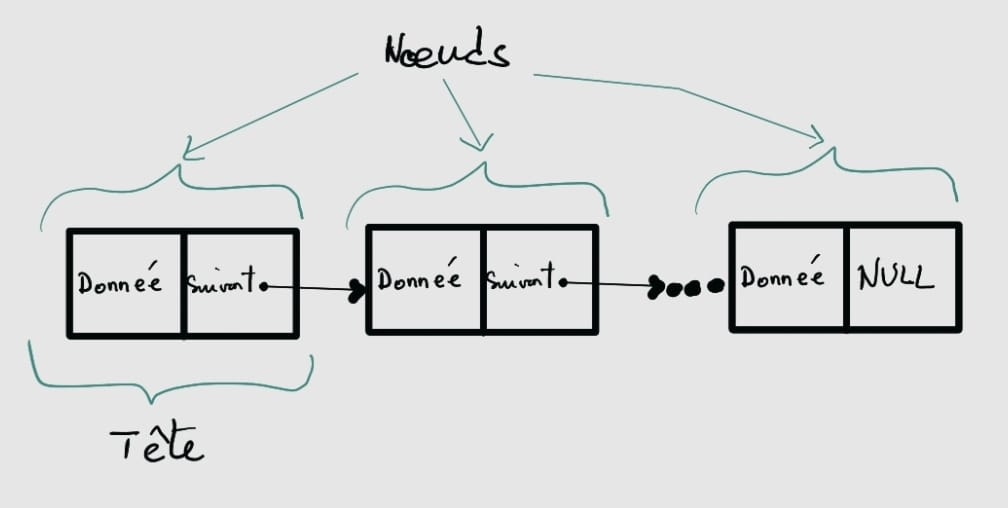
\includegraphics[width=0.8\textwidth]{image/linkedlist}
	\caption{Illustration d'une liste chaînée.}
\end{figure}

\subsection{Création d'une liste chaînée}

Pour créer une liste chaînée, commencez par définir la structure de base du nœud. Chaque nœud contient une donnée (comme un entier) et un pointeur vers le nœud suivant. Initialisez la tête de la liste à \texttt{NULL} pour indiquer qu'elle est vide.

\subsection{Insertion d'un nœud dans la liste chaînée}

Pour insérer un nœud dans une liste chaînée, vous avez deux approches principales:

\begin{itemize}
	\item \textbf{Insérer au début de la liste} : Créez un nouveau nœud, définissez ses données, puis faites pointer ce nœud vers l'ancienne tête de la liste. Mettez ensuite à jour la tête pour qu'elle pointe vers le nouveau nœud.
	
	\item \textbf{Insérer à une position spécifique} : Parcourez la liste jusqu'à la position souhaitée, créez un nouveau nœud, puis ajustez les pointeurs pour insérer le nouveau nœud à la position correcte. Si la position est zéro, insérez au début de la liste.
\end{itemize}

\subsection{Suppression d'un nœud de la liste chaînée}

Pour supprimer un nœud d'une liste chaînée, vous avez deux approches principales:

\begin{itemize}
	\item \textbf{Suppression d'un nœud par clé} : Recherchez un nœud avec une donnée spécifique. Si le nœud à supprimer est la tête de la liste, mettez à jour la tête pour qu'elle pointe vers le nœud suivant. Sinon, ajustez les pointeurs pour déconnecter le nœud du reste de la liste.
	
	\item \textbf{Suppression d'un nœud à une position spécifique} : Parcourez la liste jusqu'à la position spécifiée. Ajustez les pointeurs pour retirer le nœud à cette position. Si la position est hors limites, signalez une erreur.
\end{itemize}

%\subsection{Libération de la liste chaînée}
%
%Après avoir terminé toutes les opérations, il est essentiel de libérer toute la liste chaînée pour éviter des fuites de mémoire. Parcourez la liste, libérez chaque nœud, et assurez-vous que toutes les références à la liste sont annulées.

\subsection{Résumé}

Les listes chaînées offrent une structure flexible pour stocker des données et permettent des opérations d'insertion et de suppression efficaces. L'utilisation de pointeurs est essentielle pour manipuler la structure. Il est également crucial de gérer correctement la mémoire, surtout lors de la suppression de nœuds ou de la libération de la liste entière.

%Voici un exemple d'implémentation d'une liste chaînée en C : [Repository containing codes to be pasted here]


\section*{Exercices}
\begin{enumerate}
	\item \textbf{Création} : 
	\begin{enumerate}
		\item Écrivez un programme en C pour créer une liste chaînée contenant les nombres suivants : \texttt{10}, \texttt{20}, \texttt{30}.
		\item Affichez les éléments de la liste chaînée dans l'ordre.
	\end{enumerate}
	
	\item \textbf{Insertion} : 
	\begin{enumerate}
		\item Ajoutez un élément \texttt{40} à la fin de la liste chaînée existante.
		\item Ajoutez un élément \texttt{5} au début de la liste chaînée.
	\end{enumerate}
	
	\item \textbf{Suppression} : 
	\begin{enumerate}
		\item Supprimez l'élément \texttt{20} de la liste chaînée.
		\item Supprimez l'élément à la position \texttt{2} (indice basé sur \texttt{0}).
	\end{enumerate}
	
%	\item \textbf{Exploration} : 
%	\begin{enumerate}
%		\item Affichez tous les éléments de la liste chaînée après chaque opération d'insertion ou de suppression.
%	\end{enumerate}
\end{enumerate}


\section{Piles}

Les \emph{piles} (ou LIFO, Last In First Out) sont des structures de données où le dernier élément inséré est le premier à être retiré. Les piles sont utiles pour des opérations de retour en arrière, comme dans les navigateurs Web ou les algorithmes de récursion.

\begin{figure}[H]
	\centering
	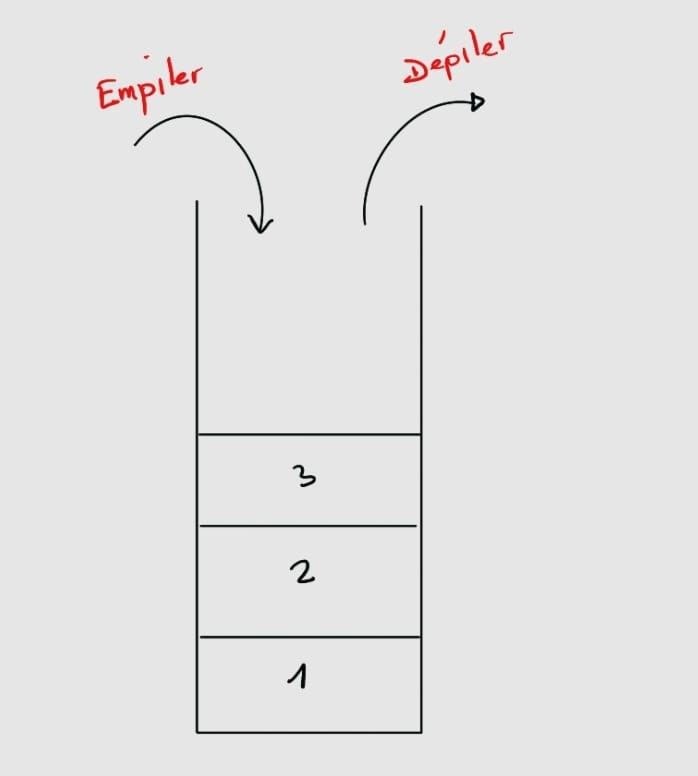
\includegraphics[width=0.5\textwidth]{image/stack} 
	\caption{Illustration d'une pile (LIFO), où le dernier élément ajouté est le premier retiré.}
\end{figure}

\subsection{Construction d'une pile}
Pour construire une pile, vous devez définir une structure qui contient des éléments (comme un tableau ou une liste) et un pointeur ou un indice qui indique le sommet de la pile. Les opérations principales associées aux piles sont l'empilage (ajout d'un élément au sommet) et le dépilage (retrait de l'élément au sommet).

\subsection{Insertion d'un élément dans une pile (empilage)}
L'empilage consiste à ajouter un élément au sommet de la pile. Pour cela, vous devez vérifier si la pile a de la place (si elle n'est pas pleine). Mettez ensuite à jour le sommet pour refléter le nouvel élément. Si vous utilisez un tableau, insérez l'élément à l'indice du sommet. Pour une pile basée sur des listes chaînées, créez un nouveau nœud et ajustez les pointeurs pour insérer le nœud au sommet.

\subsection{Suppression d'un élément dans une pile (dépilage)}
Le dépilage consiste à retirer l'élément au sommet de la pile. Comme pour l'empilage, vérifiez s'il y a des éléments dans la pile (pour éviter de dépiler une pile vide). Si la pile est vide, renvoyez une erreur ou une valeur spéciale pour indiquer qu'il n'y a rien à dépiler. Mettez ensuite à jour le sommet pour refléter le nouvel élément au sommet. Si vous utilisez un tableau, réduisez le sommet d'un indice.

\subsection{Vérification si la pile est vide}
Pour vérifier si la pile est vide, comparez le sommet à -1. Si le sommet est à -1, la pile est vide. Cette vérification est essentielle pour éviter des opérations incorrectes comme le dépilage d'une pile vide, ce qui pourrait causer des erreurs.

\subsection{Utilisations courantes des piles}
Les piles sont utilisées dans de nombreux contextes, tels que les opérations de retour en arrière, les algorithmes de récursion, et les vérifications de syntaxe. Par exemple, les piles sont utiles pour vérifier si des parenthèses sont équilibrées dans une expression mathématique ou de programmation. Elles sont également utilisées dans les navigateurs Web pour gérer l'historique des pages visitées.

\subsection{Résumé}
Les piles offrent une structure simple mais puissante pour gérer des opérations où le dernier entré est le premier à sortir. Elles sont utilisées dans de nombreux domaines informatiques, y compris les algorithmes de récursion et les éditeurs de texte. Comprendre leur fonctionnement et savoir comment les utiliser efficacement est essentiel pour tout développeur.


\section*{Exercices}
\begin{enumerate}
	\item \textbf{Création} :
	\begin{enumerate}
		\item Implémentez une pile en C à l'aide d'un tableau de taille \texttt{5}. Ajoutez les éléments suivants : \texttt{10}, \texttt{20}, \texttt{30}.
		\item Affichez les éléments actuels de la pile.
	\end{enumerate}
	
	\item \textbf{Empilage (Push)} :
	\begin{enumerate}
		\item Ajoutez deux nouveaux éléments \texttt{40} et \texttt{50} dans la pile.
		\item Essayez d’ajouter un élément \texttt{60} et gérez l’erreur si la pile est pleine.
	\end{enumerate}
	
	\item \textbf{Dépilage (Pop)} :
	\begin{enumerate}
		\item Supprimez le dernier élément inséré et affichez l’état actuel de la pile.
		\item Continuez à dépiler jusqu’à ce que la pile soit vide et gérez l’erreur si la pile est déjà vide.
	\end{enumerate}
	
	\item \textbf{Vérification} : 
	\begin{enumerate}
		\item Ajoutez une vérification pour savoir si la pile est vide ou pleine avant chaque opération.
	\end{enumerate}
\end{enumerate}


\section{Files}

Les \emph{files} (ou FIFO, First In First Out) sont des structures de données où le premier élément inséré est le premier à sortir. Contrairement aux piles, où le dernier élément ajouté est le premier à sortir, les files fonctionnent comme des files d'attente dans un magasin, où les premiers arrivés sont les premiers servis.

\begin{figure}[H]
	\centering
	 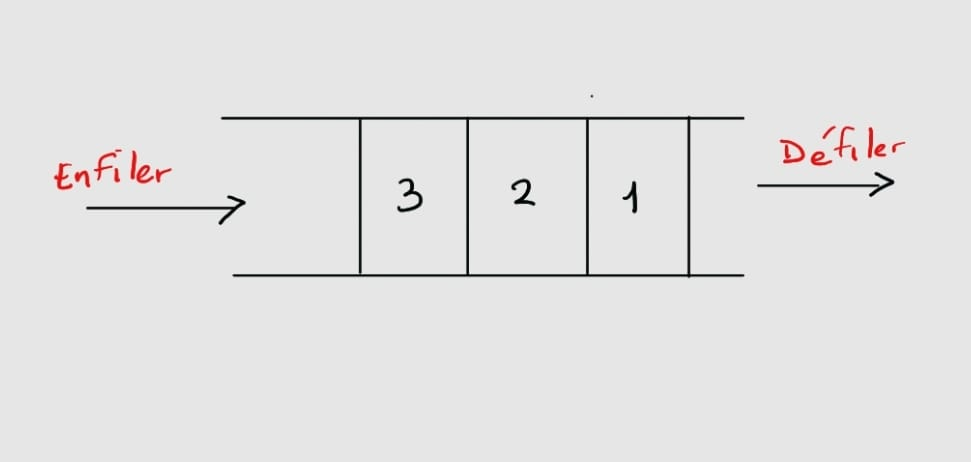
\includegraphics[width=0.8\textwidth]{image/q}  % Exemple d'illustration d'une file
	\caption{Illustration d'une file (FIFO), où le premier élément ajouté est le premier retiré.}
\end{figure}

\subsection{Construction d'une file}
Pour construire une file, définissez une structure qui contient les éléments de la file et des pointeurs vers le début (avant) et la fin (arrière). Cette structure permet des opérations d'enfilage (ajout d'un élément à l'arrière) et de défilage (retrait du premier élément).

\subsection{Insertion d'un élément dans une file (enfilage)}
L'enfilage consiste à ajouter un élément à la fin de la file. Pour cela, assurez-vous qu'il y a de l'espace pour l'élément. Si la file est vide, l'élément ajouté devient à la fois l'avant et l'arrière. Si la file contient déjà des éléments, faites pointer le dernier élément vers le nouveau, puis mettez à jour l'arrière pour indiquer le nouvel élément.

\subsection{Suppression d'un élément dans une file (défilage)}
Le défilage consiste à retirer le premier élément de la file. Avant de le retirer, vérifiez que la file n'est pas vide. Si la file est vide, renvoyez une erreur ou une valeur spéciale. Sinon, mettez à jour l'avant pour qu'il pointe vers le prochain élément, puis libérez la mémoire de l'élément supprimé.

\subsection{Vérification si la file est vide}
Pour vérifier si la file est vide, voyez si l'avant est `NULL`. Si c'est le cas, la file n'a aucun élément, ce qui signifie que vous ne pouvez pas effectuer de défilage. Cette vérification empêche des erreurs liées au défilage d'une file vide.

\subsection{Utilisations courantes des files}
Les files sont largement utilisées dans des applications informatiques où des tâches doivent être effectuées dans un ordre spécifique. Par exemple, les files sont utilisées pour la gestion des tâches, les files d'attente dans les systèmes, et les algorithmes de parcours. Elles sont également utiles pour des structures comme les queues d'impression, les files d'attente dans les réseaux, ou les systèmes d'exploitation qui gèrent des processus.

\subsection{Résumé}
Les files offrent une structure pratique pour des opérations où le premier élément inséré est le premier à sortir. Elles ont de nombreuses applications dans le monde informatique, de la gestion des tâches aux systèmes de files d'attente. Comprendre leur fonctionnement est essentiel pour travailler efficacement avec des structures FIFO.

\section*{Exercices}
\begin{enumerate}
	\item \textbf{Création} :
	\begin{enumerate}
		\item Implémentez une file en C à l'aide d’un tableau de taille \texttt{5}. Ajoutez les éléments suivants : \texttt{1}, \texttt{2}, \texttt{3}.
		\item Affichez les éléments actuels de la file.
	\end{enumerate}
	
	\item \textbf{Enfilage (Enqueue)} :
	\begin{enumerate}
		\item Ajoutez deux nouveaux éléments \texttt{4} et \texttt{5} dans la file.
		\item Essayez d’ajouter un élément \texttt{6} et gérez l’erreur si la file est pleine.
	\end{enumerate}
	
	\item \textbf{Défilage (Dequeue)} :
	\begin{enumerate}
		\item Supprimez le premier élément inséré et affichez l’état actuel de la file.
		\item Continuez à défiler jusqu’à ce que la file soit vide et gérez l’erreur si la file est déjà vide.
	\end{enumerate}
	
	\item \textbf{Exploration} :
	\begin{enumerate}
		\item Affichez tous les éléments de la file après chaque opération.
	\end{enumerate}
\end{enumerate}


\section{Arbres binaires}

Les \emph{arbres binaires} sont des structures de données où chaque nœud a au maximum deux enfants. Ils sont souvent utilisés pour des opérations de recherche, de tri, et pour implémenter des algorithmes de parcours comme le pré-ordre, l'en-ordre, et le post-ordre.

\begin{figure}[H]
	\centering
	 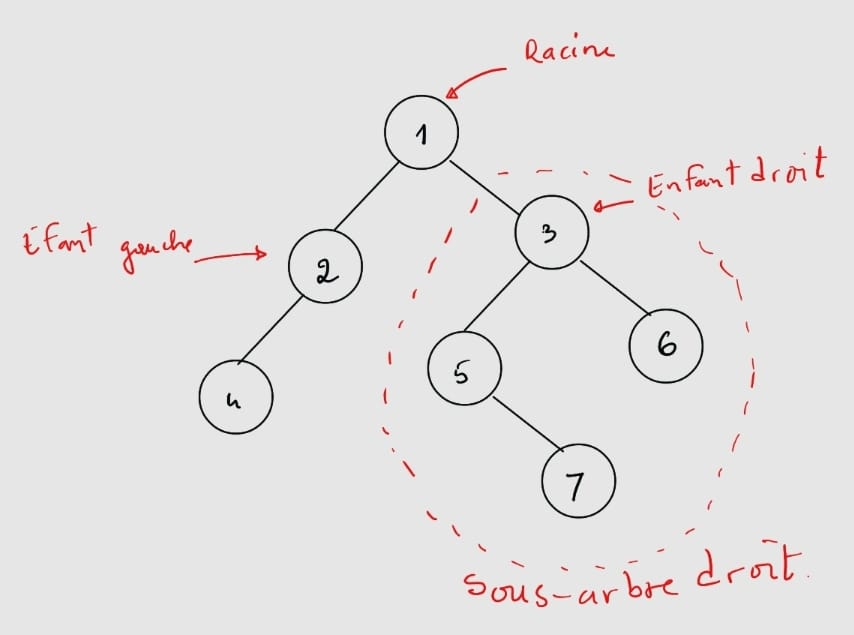
\includegraphics[width=0.8\textwidth]{image/binary_tree}  % Exemple d'illustration d'un arbre binaire
	\caption{Illustration d'un arbre binaire}
\end{figure}

\subsection{Construction d'un arbre binaire}
Pour construire un arbre binaire, définissez une structure de nœud qui contient des données (comme un entier) et des pointeurs vers les enfants gauche et droit. L'arbre binaire commence avec un seul nœud racine, et les autres nœuds sont ajoutés en fonction de leur relation avec le racine.

\subsection{Insertion dans un arbre binaire}
Pour insérer un élément dans un arbre binaire, commencez par la racine. Si le nouvel élément est plus petit que le racine, allez à gauche. S'il est plus grand, allez à droite. Continuez à descendre jusqu'à ce que vous trouviez une position vide. Ajoutez alors un nouveau nœud à cet endroit.

\subsection{Utilisations courantes des arbres binaires}
Les arbres binaires sont largement utilisés dans des algorithmes informatiques. Ils permettent des opérations de recherche rapides car les éléments peuvent être trouvés sans parcourir tout l'arbre. Les arbres binaires peuvent être utilisés pour des opérations comme la recherche binaire, le tri d'arbres, et le parcours de différentes manières (pré-ordre, en-ordre, post-ordre).

\subsection{Algorithmes de parcours des arbres binaires}

Les algorithmes de parcours des arbres binaires permettent d'explorer ou de traverser les arbres de différentes manières. Les méthodes courantes de parcours sont le parcours en-ordre, le parcours pré-ordre, et le parcours post-ordre.

\begin{enumerate}[label=\alph*)]
	\item \textbf{Parcours en-ordre}
	
	Le parcours en-ordre consiste à visiter les nœuds d'un arbre binaire dans un ordre spécifique : d'abord le sous-arbre gauche, puis le nœud actuel, et enfin le sous-arbre droit. Cette méthode est souvent utilisée pour obtenir les éléments dans un ordre trié.
	
	- Fonctionnement : Commencez par le sous-arbre gauche, puis visitez le nœud actuel, et terminez par le sous-arbre droit. Cela donne les éléments de l'arbre dans un ordre croissant.
	
	\item \textbf{Parcours pré-ordre}
	
	Le parcours pré-ordre visite d'abord le nœud actuel, puis les sous-arbres gauche et droit. Il est souvent utilisé pour copier des arbres binaires ou pour créer des représentations pré-ordre.
	
	- Fonctionnement : Visitez le nœud actuel, puis parcourez le sous-arbre gauche, puis le sous-arbre droit. Cela peut être utilisé pour recréer l'arbre ou explorer tous les nœuds.
	
	\item \textbf{Parcours post-ordre}
	
	Le parcours post-ordre commence par les sous-arbres gauche et droit, puis visite le nœud actuel. Cette méthode est souvent utilisée pour supprimer des arbres ou pour des opérations nécessitant une évaluation de bas en haut.
	
	- Fonctionnement : Commencez par le sous-arbre gauche, puis le sous-arbre droit, et enfin visitez le nœud actuel. Ce parcours est utile pour des opérations de suppression ou de nettoyage d'arbre.
	
\end{enumerate}

Les algorithmes de parcours des arbres binaires ont des applications variées. Le parcours en-ordre est idéal pour obtenir des éléments dans un ordre trié, le pré-ordre est utilisé pour copier ou recréer des arbres, et le post-ordre est souvent utilisé pour des opérations de suppression ou de nettoyage. Comprendre ces différentes méthodes de parcours est essentiel pour travailler avec des arbres binaires et résoudre des problèmes complexes d'arborescence.


\subsection{Résumé}
Les arbres binaires sont des structures de données polyvalentes, idéales pour des opérations de recherche et de tri. Ils permettent des algorithmes efficaces pour parcourir des données de manière structurée. Comprendre comment insérer des nœuds et utiliser des arbres binaires est crucial pour travailler avec des structures de données avancées.

\section*{Exercices}
\begin{enumerate}
	\item \textbf{Création (Complétez le code)} :
	\begin{enumerate}
		\item Le code ci-dessous initialise une structure pour un nœud d'arbre binaire. Complétez-le en ajoutant la fonction \texttt{createNode} pour allouer de la mémoire et initialiser un nœud.
		\begin{verbatim}
			struct Node {
				int data;
				struct Node* left;
				struct Node* right;
			};
			
			--- Ajoutez la fonction createNode ici ---
			
			int main() {
				struct Node* root = createNode(50);
				printf("Racine créée avec succès : %d", root->data);
				return 0;
			}
		\end{verbatim}
	\end{enumerate}
	
	\item \textbf{Insertion (Ajoutez les lignes manquantes)} :
	\begin{enumerate}
		\item Complétez la fonction d'insertion dans un arbre binaire. Ajoutez les conditions pour insérer un nœud à gauche ou à droite.
		\begin{verbatim}
			struct Node* insert(struct Node* root, int data) {
				if (root == NULL) {
					return createNode(data);
				}
				if (data < root->data) {
					// Ligne manquante pour insérer à gauche
				} else {
					// Ligne manquante pour insérer à droite
				}
				return root;
			}
		\end{verbatim}
		\item Testez votre fonction en insérant les éléments suivants : \texttt{30}, \texttt{70}, \texttt{20}.
	\end{enumerate}
	
	\item \textbf{Parcours (Complétez le code)} :
	\begin{enumerate}
		\item Complétez la fonction de parcours en pré-ordre en remplissant la logique pour visiter les enfants gauche et droit :
		\begin{verbatim}
			void preOrder(struct Node* root) {
				if (root != NULL) {
					printf("%d ", root->data);
					--- Ajoutez l'appel pour visiter l'enfant gauche ---
					--- Ajoutez l'appel pour visiter l'enfant droit ---
				}
			}
		\end{verbatim}
		\item Affichez les éléments de l’arbre en utilisant votre fonction.
	\end{enumerate}
	
	\item \textbf{Suppression (Avec guide)} :
	\begin{enumerate}
		\item Ajoutez la logique pour supprimer un nœud ayant deux enfants :
		\begin{verbatim}
			struct Node* deleteNode(struct Node* root, int data) {
				if (root == NULL) return root;
				if (data < root->data) {
					root->left = deleteNode(root->left, data);
				} else if (data > root->data) {
					root->right = deleteNode(root->right, data);
				} else {
					if (root->left == NULL && root->right == NULL) {
						free(root);
						return NULL;
					}
					// Ajoutez ici la logique pour trouver le successeur en-ordre
				}
				return root;
			}
		\end{verbatim}
		\item Supprimez l’élément \texttt{70} de l’arbre existant et affichez les éléments en parcours en-ordre.
	\end{enumerate}
\end{enumerate}



\section{Graphes}

Les \emph{graphes} sont des structures de données composées de nœuds (ou sommets) et d'arêtes (les connexions entre les nœuds). Les graphes peuvent être orientés ou non orientés. Dans un graphe orienté, les arêtes ont une direction (comme une flèche). Dans un graphe non orienté, les arêtes n'ont pas de direction particulière. Les graphes sont utilisés pour résoudre des problèmes complexes comme la recherche des plus courts chemins, la détection de cycles, ou le partitionnement.

\begin{figure}[H]
	\centering
	 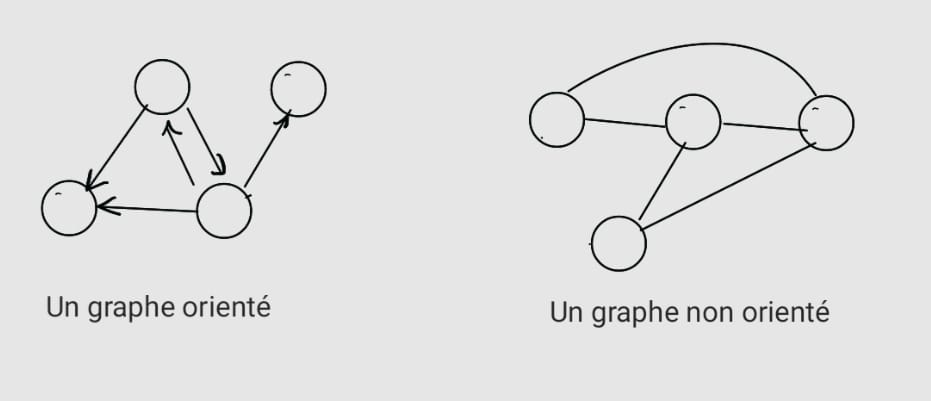
\includegraphics[width=0.8\textwidth]{image/graph}  % Exemple d'illustration d'un graphe
	\caption{Exemples des deux types de graphes}
\end{figure}

\subsection{Construction d'un graphe}
Pour construire un graphe, vous devez définir une structure qui contient une liste de sommets et des arêtes qui les relient. Les graphes peuvent être implémentés de différentes manières, comme avec des listes d'adjacence ou des matrices d'adjacence.

Dans le cas des listes d'adjacence, chaque sommet a une liste de connexions vers d'autres sommets. Les graphes peuvent être orientés (avec des flèches pour indiquer la direction des arêtes) ou non orientés (où les connexions sont bidirectionnelles). Pour construire un graphe, initialisez le nombre de sommets et allouez de la mémoire pour chaque liste d'adjacence.

\subsection{Ajout d'arêtes (liens) dans un graphe}
Pour ajouter des arêtes dans un graphe, vous devez d'abord déterminer les sommets que vous voulez relier. Si le graphe est orienté, assurez-vous de respecter la direction des arêtes. Pour un graphe non orienté, ajoutez des connexions bidirectionnelles. 

Dans le cas des listes d'adjacence, créez un nouveau nœud pour chaque connexion, puis ajoutez-le à la liste du sommet correspondant. Assurez-vous que les arêtes sont correctement ajoutées pour éviter les erreurs de connexion.

\subsection{Utilisations courantes des graphes}
Les graphes sont utilisés dans de nombreux domaines informatiques. Ils permettent de modéliser des relations complexes entre des entités. Par exemple, les graphes peuvent représenter des réseaux de transport, des relations sociales, ou des connexions informatiques. Les graphes sont également utiles pour des algorithmes de parcours comme la recherche en profondeur (DFS) ou la recherche en largeur (BFS).

Les graphes peuvent résoudre des problèmes comme la recherche du plus court chemin, la détection de cycles, et la recherche de composants connexes. Comprendre leur fonctionnement est essentiel pour travailler avec des structures de données avancées.

\subsection{Algorithmes de parcours de graphes}

Les algorithmes de parcours de graphes permettent d'explorer ou de traverser les graphes de différentes manières. Les méthodes courantes de parcours incluent la recherche en profondeur (DFS) et la recherche en largeur (BFS).

\begin{enumerate}[label=\alph*)]
	\item \textbf{Recherche en profondeur (DFS -- [Depth First Search])}
	
	DFS explore le graphe en suivant chaque branche aussi loin que possible avant de revenir en arrière. Elle utilise une pile pour mémoriser les nœuds visités. DFS est souvent utilisée pour détecter des cycles, trouver des composants connexes, ou résoudre des problèmes de recherche de chemins.
	
	- Fonctionnement : DFS commence à partir d'un nœud et explore tous ses voisins. Ensuite, il passe au nœud suivant non visité, poursuivant ainsi la profondeur jusqu'à ce qu'il n'y ait plus de nœuds à visiter. Puis, il revient en arrière pour explorer d'autres chemins.
	
	\item \textbf{Recherche en largeur (BFS -- [Breadth First Search])}
	
	BFS explore le graphe couche par couche, en visitant tous les voisins d'un nœud avant de passer au suivant. Elle utilise une file pour mémoriser les nœuds à visiter. BFS est couramment utilisée pour trouver des plus courts chemins dans des graphes non pondérés ou pour des problèmes de recherche de niveaux.
	
	- Fonctionnement : BFS commence par le premier nœud et visite tous ses voisins. Ensuite, il passe aux voisins de ces voisins, touchant tous les nœuds au même niveau avant de passer au niveau suivant.
	
\end{enumerate}

Les algorithmes de parcours de graphes ont des applications variées. DFS est utilisé pour des analyses approfondies, comme la recherche de cycles ou de chemins profonds, tandis que BFS est idéal pour des analyses en surface, comme trouver des connexions courtes ou explorer des niveaux. Ces algorithmes sont essentiels pour résoudre des problèmes complexes de graphes.


\subsection{Résumé}

Les graphes sont des structures de données puissantes qui permettent de modéliser des connexions entre des sommets. Ils sont utilisés dans de nombreux domaines, comme les réseaux informatiques, les systèmes de transport, ou l'analyse sociale. Les graphes peuvent être orientés (où les arêtes ont une direction) ou non orientés (où les connexions sont bidirectionnelles).

Les algorithmes de parcours comme la recherche en profondeur (DFS) et la recherche en largeur (BFS) sont des outils essentiels pour travailler avec des graphes. DFS explore les graphes en profondeur, tandis que BFS explore les graphes en largeur, offrant des applications diverses pour des problèmes complexes.

Les graphes peuvent résoudre des problèmes tels que la recherche des plus courts chemins, la détection de cycles, ou la recherche de composants connexes. Ils permettent également de modéliser des systèmes complexes avec des connexions multiples. La compréhension des graphes, de leurs applications et des algorithmes de parcours est essentielle pour résoudre des problèmes avancés en informatique.



\section*{Exercices}
\begin{enumerate}
	\item \textbf{Création (Complétez le code)} :
	\begin{enumerate}
		\item Complétez la fonction pour créer un graphe. Ajoutez la logique pour initialiser chaque liste d’adjacence.
		\begin{verbatim}
			struct Graph* createGraph(int vertices) {
				struct Graph* graph = malloc(sizeof(struct Graph));
				graph->numVertices = vertices;
				graph->adjLists = malloc(vertices * sizeof(struct Node*));
				for (int i = 0; i < vertices; i++) {
					--- Ajoutez la ligne pour initialiser chaque liste d'adjacence ---
				}
				return graph;
			}
		\end{verbatim}
	\end{enumerate}
	
	\item \textbf{Ajout d’arêtes (Complétez la fonction)} :
	\begin{enumerate}
		\item Complétez la fonction pour ajouter une arête entre deux sommets dans un graphe non orienté :
		\begin{verbatim}
			void addEdge(struct Graph* graph, int src, int dest) {
				struct Node* newNode = malloc(sizeof(struct Node));
				newNode->vertex = dest;
				newNode->next = --- Ajoutez ici pour lier au sommet source ---
				graph->adjLists[src] = newNode;
				
				// Ajouter la même logique pour dest -> src
			}
		\end{verbatim}
		\item Ajoutez des arêtes entre les sommets \texttt{A}, \texttt{B}, \texttt{C}, et \texttt{D}.
	\end{enumerate}
	
	\item \textbf{Recherche en largeur (Complétez le code)} :
	\begin{enumerate}
		\item Ajoutez la logique pour visiter tous les voisins d’un sommet dans la fonction BFS :
		\begin{verbatim}
			void BFS(struct Graph* graph, int startVertex) {
				int visited[graph->numVertices];
				for (int i = 0; i < graph->numVertices; i++) visited[i] = 0;
				
				struct Queue* queue = createQueue();
				visited[startVertex] = 1;
				enqueue(queue, startVertex);
				
				while (!isEmpty(queue)) {
					int currentVertex = dequeue(queue);
					printf("%d ", currentVertex);
					
					struct Node* temp = graph->adjLists[currentVertex];
					while (temp) {
						int adjVertex = temp->vertex;
						if (!visited[adjVertex]) {
							visited[adjVertex] = 1;
							--- Ajoutez ici la logique pour mettre en file le sommet voisin ---
						}
						temp = temp->next;
					}
				}
			}
		\end{verbatim}
		\item Testez la fonction BFS à partir du sommet \texttt{A}.
	\end{enumerate}
	
	\item \textbf{Exploration (Ajoutez des vérifications)} :
	\begin{enumerate}
		\item Ajoutez une fonction pour vérifier si une arête existe entre deux sommets :
		\begin{verbatim}
			int edgeExists(struct Graph* graph, int src, int dest) {
				struct Node* temp = graph->adjLists[src];
				while (temp != NULL) {
					if (temp->vertex == dest) {
						--- Retournez une valeur indiquant que l'arête existe ---
					}
					temp = temp->next;
				}
				--- Retournez une valeur indiquant que l'arête n'existe pas ---
			}
		\end{verbatim}
		\item Testez la fonction pour les sommets \texttt{A} et \texttt{D}.
	\end{enumerate}
\end{enumerate}

	\chapter{Applications d'algorithmes en IA}

\section{Introduction}
L'intelligence artificielle repose sur des algorithmes sophistiqués pour prendre des décisions, analyser des données et résoudre des problèmes complexes. Ce chapitre explore les algorithmes populaires de l'IA en mettant l’accent sur leur fonctionnement étape par étape et sur des exemples concrets qui illustrent leur application.

\section{Algorithmes d'Apprentissage Supervisé}

\subsection{Régression Linéaire}
La \textbf{régression linéaire} est utilisée pour prédire une valeur numérique continue (comme un prix ou une température) en fonction d'une ou plusieurs variables.

\begin{itemize}
	\item \textbf{Idée de base} : Imaginez un nuage de points sur un graphique où l'axe $x$ représente une variable (par exemple, la taille d’une maison) et l'axe $y$ représente le résultat (comme le prix de la maison). La régression linéaire cherche à tracer une ligne qui passe le plus près possible de ces points.
	\item \textbf{Étapes de l’algorithme} :
	\begin{enumerate}
		\item \textbf{Préparer les données} : Regroupez les données en paires $(x, y)$.
		\item \textbf{Déterminer l’équation} : Une ligne est définie par $y = ax + b$.
		\item \textbf{Ajuster la ligne} : Trouvez $a$ et $b$ pour minimiser l’erreur.
		\item \textbf{Prédire} : Utilisez $y = ax + b$ pour de nouvelles valeurs de $x$.
	\end{enumerate}
\end{itemize}

\begin{table}[h]
	\centering
	\caption{Données pour la régression linéaire}
	\begin{tabular}{|c|c|}
		\hline
		Surface (m²) & Prix (MGA) \\ \hline
		50           & 70,000,000 \\ \hline
		75           & 95,000,000 \\ \hline
		100          & 130,000,000 \\ \hline
	\end{tabular}
\end{table}

\begin{figure}[h]
	\centering
	\begin{tikzpicture}
		% Axes
		\draw[->] (0,0) -- (5,0) node[right] {Surface (m²)};
		\draw[->] (0,0) -- (0,5) node[above] {Prix (MGA)};
		
		% Gridlines
		\draw[gray!10, thin] (0,0) grid (5,5);
		
		% Points
		\filldraw[blue] (1,1) circle (2pt) node[below left] {};
		\filldraw[blue] (2.5,2.3) circle (2pt) node[below right] {};
		\filldraw[blue] (4,4) circle (2pt) node[below right] {};
		\filldraw[blue] (1,0) circle (1pt) node[below right] {50};
		\filldraw[blue] (2.5,0) circle (1pt) node[below right] {75};
		\filldraw[blue] (4,0) circle (1pt) node[below right] {100};
		
		% Regression line
		\draw[red, thick] (0.5,0.5) -- (4.5,4.5) node[right] {Ligne de régression};
	\end{tikzpicture}
	\caption{Régression linéaire sur des données simulées.}
\end{figure}

\section*{Exercice : Implémenter la Régression Linéaire}
\begin{enumerate}
	\item  Écrivez un programme en C qui :  
\begin{itemize}
	\item Accepte les paires $(x, y)$ en entrée.  
	\item Calcule les coefficients $a$ et $b$.  
	\item Prédit $y$ pour une nouvelle valeur $x$.  
\end{itemize}
\item  Utilisez les données du tableau ci-dessus et prédisez $y$ pour $x = 80$.  
\end{enumerate}

\subsection{Régression Logistique}
La \textbf{régression logistique} est utilisée pour prédire une probabilité binaire, comme "oui/non" ou "succès/échec".

\begin{itemize}
	\item \textbf{Idée de base} : Contrairement à la régression linéaire, la régression logistique utilise une \textit{fonction sigmoïde} pour transformer un score $z$ en une probabilité :
	\[
	P = \frac{1}{1 + e^{-z}}
	\]
	\item \textbf{Étapes de l’algorithme} :
	\begin{enumerate}
		\item Calculez $z$ avec $z = a \cdot x + b$.
		\item Appliquez la fonction sigmoïde pour obtenir $P$.
		\item Comparez $P$ avec un seuil (e.g., 0,5) pour décider "oui" ou "non".
	\end{enumerate}
\end{itemize}

\begin{table}[h]
	\centering
	\caption{Exemple pour la régression logistique}
	\begin{tabular}{|c|c|c|}
		\hline
		Temps (minutes) & Pages visitées & $z$ \\ \hline
		12              & 7              & $z = 2.3$ \\ \hline
	\end{tabular}
\end{table}

\begin{figure}[h]
	\centering
	\begin{tikzpicture}
		% Axes
		\draw[->] (-5,0) -- (5,0) node[right] {Score $z$};
		\draw[->] (0,0) -- (0,5) node[above] {Probabilité $P$};
		\draw[dashed] (-5, 4) -- (5,4) node[right] { $P=1$};
		% Sigmoid curve
		\draw[blue, thick, smooth, domain=-5:5, samples=100] plot (\x,{4/(1 + exp(-\x))});
		
		% Threshold line
		\draw[dashed] (-5,2) -- (5,2) node[right] {Seuil $P = 0.5$};
	\end{tikzpicture}
	\caption{Courbe sigmoïde pour la régression logistique.}
\end{figure}

\section*{Exercice : Implémenter la Régression Logistique}
\begin{enumerate}
	\item  Écrivez un programme en C qui :  
\begin{itemize}
	\item Calcule $z$ pour une valeur donnée.  
	\item Transforme $z$ en $P$ à l’aide de la fonction sigmoïde.  
	\item Compare $P$ avec un seuil pour afficher "Oui" ou "Non".  
\end{itemize}
\item Utilisez les données du tableau ci-dessus et prédisez si le client achètera.
\end{enumerate}

\subsection{Clustering avec K-means}
L’algorithme \textbf{K-means} regroupe des données en plusieurs groupes appelés \textit{clusters}.

\begin{itemize}
	\item \textbf{Idée de base} : Divisez les données en $K$ groupes, chaque groupe ayant un centre (\textit{centroïde}).
	\item \textbf{Étapes de l’algorithme} :
	\begin{enumerate}
		\item Choisissez $K$ centroïdes aléatoires.
		\item Assignez chaque point au centroïde le plus proche.
		\item Recalculez les centroïdes en prenant la moyenne des points.
		\item Répétez jusqu'à ce que les centroïdes ne changent plus.
	\end{enumerate}
\end{itemize}

\begin{table}[h]
	\centering
	\caption{Données pour K-means}
	\begin{tabular}{|c|c|}
		\hline
		Point & Coordonnées $(x, y)$ \\ \hline
		A     & (1, 2)              \\ \hline
		B     & (3, 4)              \\ \hline
		C     & (5, 6)              \\ \hline
		D     & (8, 9)              \\ \hline
	\end{tabular}
\end{table}

\begin{figure}[h]
	\centering
	\begin{tikzpicture}
		% Axes
		\draw[->] (0,0) -- (6,0) node[right] {Caractéristique 1};
		\draw[->] (0,0) -- (0,6) node[above] {Caractéristique 2};
		
		% Points
		\filldraw[red] (1,1) circle (2pt) node[below left] {A};
		\filldraw[red] (1.5,1.5) circle (2pt) node[below right] {B};
		\filldraw[blue] (4,4) circle (2pt) node[below] {C};
		\filldraw[blue] (4.5,4.5) circle (2pt) node[above right] {D};
		
		% Centroids
		\filldraw[black] (1.25,1.25) circle (3pt) node[above left] {C1};
		\filldraw[black] (4.25,4.25) circle (3pt) node[below right] {C2};
	\end{tikzpicture}
	\caption{Clustering K-means avec deux clusters.}
\end{figure}

\section*{Exercice : Implémenter K-means}
\begin{enumerate}
	\item  Écrivez un programme en C qui :  
\begin{itemize}
	\item Accepte une liste de points $(x, y)$.  
	\item Initialise 2 centroïdes aléatoires.  
	\item Assigne chaque point au centroïde le plus proche.  
	\item Recalcule les centroïdes et affiche les groupes finaux.  
\end{itemize}
\item  Utilisez les données du tableau ci-dessus. 
\end{enumerate}


%\chapter{Structures de donn\'ees fondamentales}
%\chapter{Algorithmes de recherche et de tri}
%\chapter{Complexité algorithmique}

\nocite{*}
\bibliographystyle{plain}
\bibliography{reference}	
\end{document}